\chapter{Redes y Casuísticas}\label{S:tema_3}
Este tema resume y expone ejemplos llevados a cabo en la prueba de concepto de redes para la oficina virtual. Es de especial interés para comprender el detalle realizado la lectura del Anexo \ref{S:anexo_D}.

\section{VPN e intranet}
Primeramente hemos de entender que siempre existe una “red común”, por lo tanto ya sea como freelance en mi oficina en casa, o la sede física de una pequeña pyme o una gran oficina en un edificio de cristal en el centro metropolitano, o una red en un cloud siempre existe una \textbf{red principal}.

\subsection{Objetivos de VPN}
Normalmente los servicios internos están accesibles dentro de esta red y bloqueados externamente. Por lo tanto tenemos múltiples intereses para implementar una VPN o virtual private network, comúnmente llamadas intranet, que nos permita el acceso a esta red interna:
\begin{itemize}
    \item Conexión directa con otros elementos de la VPN, es la funcionalidad básica de una red, permite interconectar pc, impresoras o varias personas, pero usando una interfaz virtual, es decir, cada uno usando como soporte su LAN-real.\textbf{ Especialmente interesante para utilizar elementos de control remoto} o monitorización.

    \item Conexión entre redes, en muchos casos puede ser de interés que múltiples LAN (múltiples sedes) sean también accesibles entre sí mediante la red principal sin necesidad de ser expuestas a internet o alquilar un cable-túnel a un proveedor de telecomunicaciones.
    \item DNS, monitorizado y filtrado. Especialmente útil para monitorizar. Usualmente las redes tienen su propio dns, que aparte de añadir servicios interno, permite filtrar llamadas dns o implementar otros mecanismo útiles anti spam\cite{c_pi_hole}.
    \item Salida predeterminada. En algunos casos nos interesa que la IP desde la que salimos sea nuestra red principal, ya sea por temas de legalidad, accesos concedidos u otros servicios que filtran por ubicación o ip.
\end{itemize}

Para entender adecuadamente cómo funcionan las VPN hay que refrescar conceptos básicos de Redes véase anexo \ref{S:anexo_D} tales como 'NAT', 'Enrutado', 'DNS', 'proxy reverse', así como elementos utilizados en nuestro despliegue. .

\subsection{Tipo de enlaces VPN}

En base a la topología o complejidad o tecnología utilizada existen diferentes tipos de enlaces, en este trabajo asumimos siempre VPN a niveles L2 o L3 de la capa OSI\cite{c_osi}, es decir equivalentes a una red cableada.

\begin{figure}[!htb]
\begin{center}
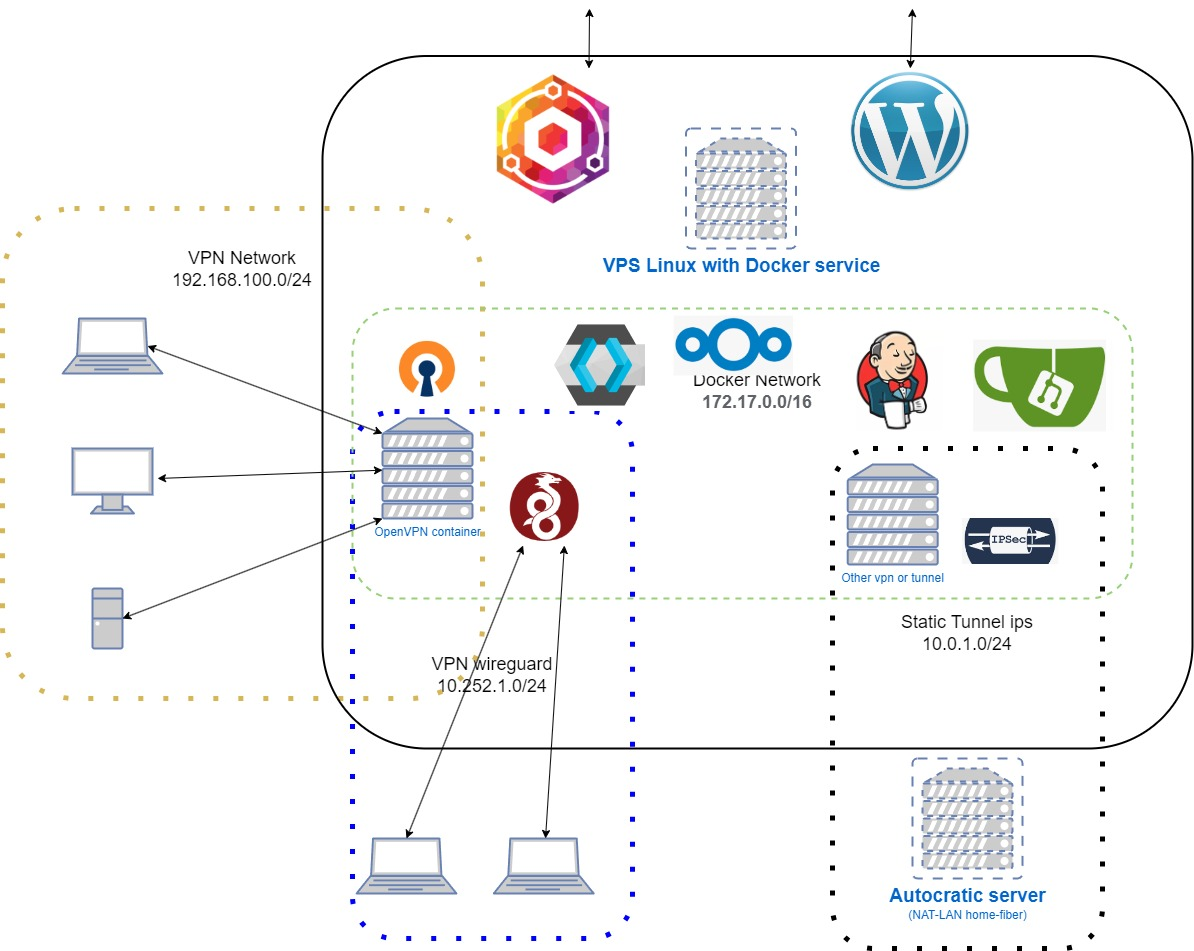
\includegraphics[width=0.9\textwidth]{./figuras/entorno_redes}
\caption{Casuística de interés de VPN - VPS.}
\label{F:entorno_redes}
\end{center}
\end{figure}

\begin{itemize}
    \item Túneles P2P, es decir, conexiones puntuales para interconectar redes o servidores. Usualmente estáticas, utilizadas como red de transporte troncal. Es una mono-red  ya que es un único enlace entre dos nodos y se les denomina como túneles ya que una vez entra el tráfico en ellas sale en el destino.
    \item VPN como servicio-salida a internet, aunque puede ser entendido como un nodo central de enlaces p2p, formando una red al re-enrutar tráfico en el nodo central, su objetivo radica como puerta de enlace para conectar clientes externos. Su objetivo principal es acceder a intranets y geo-localizar el cliente dentro de la intranet, saliendo al exterior con IP y legalidad del servidor VPS. 
    \item Conectar o exponer elementos de manera sencilla sin necesidad de IP pública, pre-configurado de nat-reverse y firewall. Se utiliza un cliente de una conexión reversa a una VPN como servicio-salida, evitando problemas intermedios tales como NAT, firewall, CG-NAT\cite{c_cg_nat} de la red proveedora de conectividad, el objetivo en este caso no es el enrutado sobre la vpn, sino lo contrario, la exposición de un servicio en la propia VPN a internet a través de IP pública del VPS que ofrece la VPN.
    \item Seguridad y compartimentación, la red así como las intranet son una capa más de seguridad por aislamiento al cifrar una comunicación y limitar el acceso a las comunicaciones e imponer una barrera de acceso a recursos únicamente ofrecidos dentro de la intranet.
\end{itemize}


\section{Casuísticas de interés}
Obviando la conexión directa de elementos públicos o privados (detrás de NAT), o la definición propia de VPN para usar dicha red en nuestros objetivos existen un conjunto de situaciones que se resuelven con una implementación por defecto de VPN.

\subsection{ Interconexión de redes privadas por VPN}
Este caso es de interés muy habitual, múltiples LANs, especialmente si son redes de oficinas regionales, desean estar interconectadas de manera privada, es decir equivalente a interconectadas por cable, para permitir acceder a los diferentes servicios o clientes de cada una de ellas.
\begin{figure}[!htb]
\begin{center}
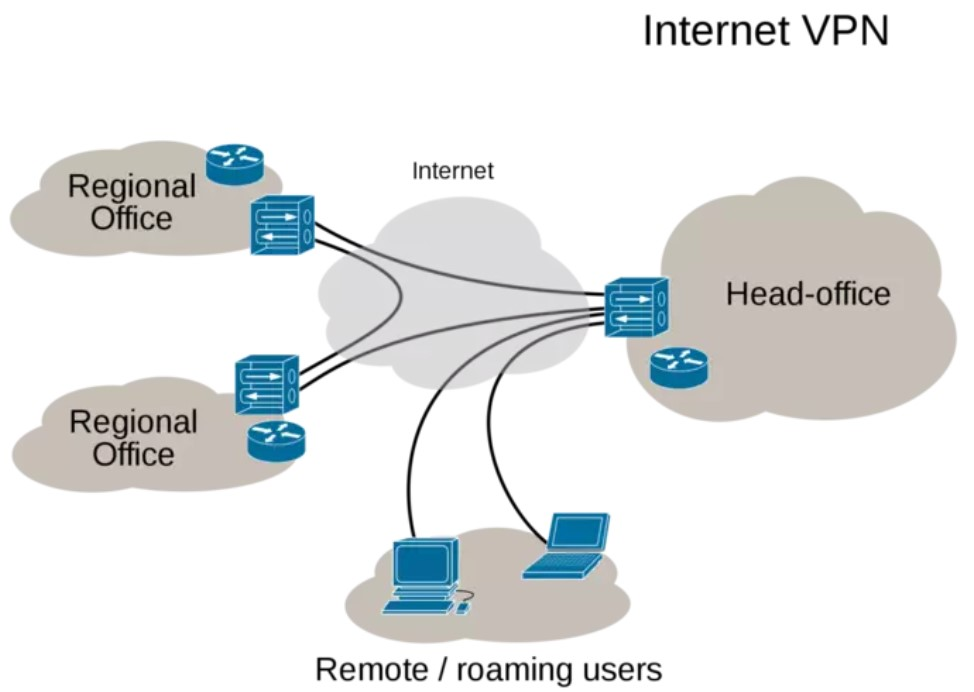
\includegraphics[width=0.75\textwidth]{./figuras/vpn_network_link}
\caption{Diagrama interconexión de redes por VPN\cite{i_redes_sedes}.}
\label{F:vpn_network_link}
\end{center}
\end{figure}
Se define una VPN, la cual actúa como red de transporte en forma de estrella, e incluye unas reglas de enrutado para anunciar y permitir la comunicación entra Lan - VPN- Lan. Véase anexo \ref{S:enrutado_sedes} con un caso detallado y explicado.

Los principales servicios más beneficiados son IT (soporte), servidores de almacenamiento en red y el uso de protocolos de comunicación (FTP, PING ..) entre elementos de ambas redes.

Un punto importante de la interconexión de LANs y VPS es el uso extensivo de captación de imágenes de seguridad y sensores tales como cámaras ip, sensores wifi o gateways de sensores (zigbee, z-wave o bluetooth) ya que son sistemas que suelen estar aislados a LANs no expuestas y no accesibles.

Se debe entender que no es necesario instalar un cliente VPN en cada elemento de la LAN, sino definir aquel elemento que “enruta” el tráfico por la vpn o utilizar un router con cliente VPN ( véase anexo \ref{S:enrutado_sedes}).

\subsection{ Múltiples capas de VPN}\label{S:doble_layer}
Desde la perspectiva de seguridad pero especialmente para la separación de conocimiento o grupos de trabajo existe la necesidad de una VPN principal (intranet) para acceder a los servicios esenciales y la conectividad una vez ya dentro de la intranet de otras VPN para redes concretas no expuestas por el VPS. Esto también aplica a la gestión UI de la propia VPN-layer2 evitando puntos de ataque por no estar expuesta a internet.

\begin{figure}[!htb]
\begin{center}
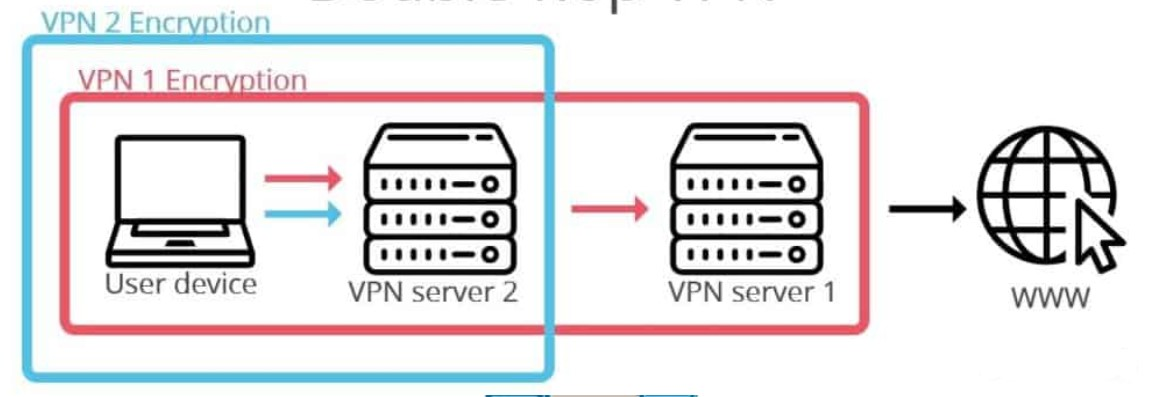
\includegraphics[width=0.75\textwidth]{./figuras/vpn_ultiples_layers}
\caption{VPN multi-salto, multi-capa.}
\label{F:vpn_ultiples_layers}
\end{center}
\end{figure}

De especial interés también puede ser el uso de una o mas tecnologías vpn, combinando diferentes capas y tecnologías.

\subsection{DNS filtro y espejos.}

Un servicio DSN-proxy interno es de especial necesidad para ofrecer una interfaz intuitiva al acceso de los servicios internos, así como filtro de seguridad capaz de filtrar publicidad o accesos web inseguras o en black list similares a pihole\cite{c_pi_hole}.
\begin{figure}[!htb]
\begin{center}
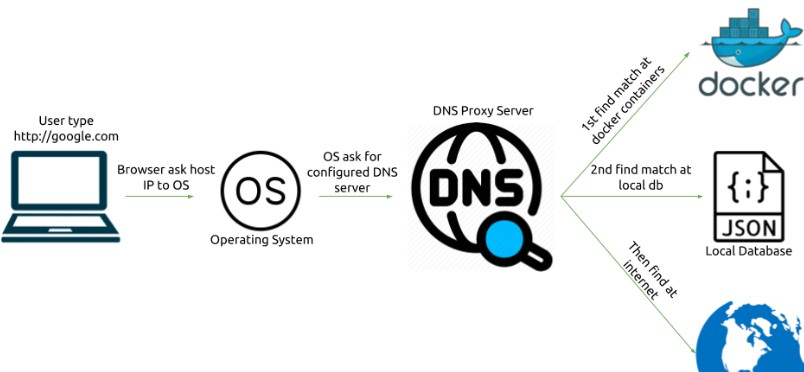
\includegraphics[width=0.8\textwidth]{./figuras/dns-proxy.jpg}
\caption{Diagrama DNS proxy\cite{i_dns}.}
\label{F:dns_proxy}
\end{center}
\end{figure}
Dentro de la VPN es de especial utilidad puesto que los servicios dockerizados no expuestos no tiene una IP estática, por consiguiente la asignación de un DNS interno que contenga los dominios internos dentro de la VPN es algo necesario (véase anexo \ref{S:dns}).

Finalmente existe la necesidad de creación de repositorios espejos, es decir, se bloquea el acceso a repositorios de uso común como dockerhub, maven, node etc.. y se crea un repositorio interno espejo que cachea o generan repositorios “aptos” (aprobados por seguridad o pendientes de auditar), para su uso interno como espejo de los públicos.

\subsection{Exposición externa vía VPS}
A veces no disponer de recursos, una ip pública en una sede o restricciones legales es un impedimento para ejecutar servicios en dicho lugar geográfico.
En estos casos se utiliza un elemento publico adecuado (IP y ubicación) para tunelar trafico (vía VPN) a nuestros recursos privados.
\begin{figure}[!htb]
\begin{center}
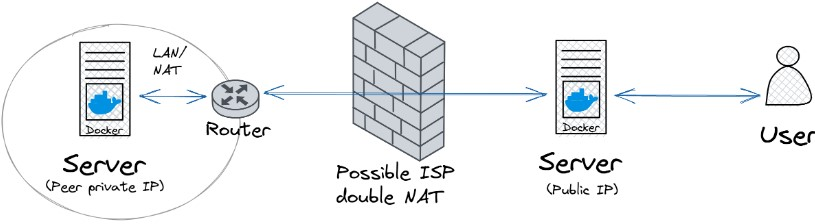
\includegraphics[width=1\textwidth]{./figuras/tunnel_resources.jpg}
\caption{Conexión a recursos detrás de CG-NAT / Firewall o NAT.}
\label{F:tunnel_resources}
\end{center}
\end{figure}

Por otra parte la exposición de los recursos detrás del tunel pueden ser expuestos utilizando una técnica de "proxy reverse", que es también utilizada como automatización de multi-dominio en el propio servidor VPS. Otro interés puede ser la atenuación de ataques o recopilación de estadísticas si nuestra nube de gran potencia pasa por proxy en un VPS, fácilmente bloqueable o parapetado con un firewall.

\begin{figure}[!htb]
\begin{center}
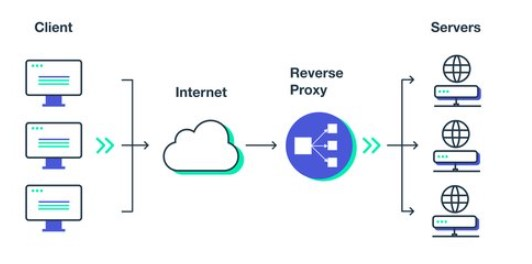
\includegraphics[width=0.8\textwidth]{./figuras/reverse_proxy.jpg}
\caption{Reverse proxy diagram.}
\label{F:reverse_proxy}
\end{center}
\end{figure}

 Un ejemplo simple es la reconversión de una vieja bodega en un pequeño cluster de servidores para un proveedor de pymes. Probablemente el aislamiento y temperatura de la bodega, es idóneo para la refrigeración y uso continuado de los servidores, así como la utilización de recursos verdes para generación eléctrica o refrigeración activa fácilmente amortizables. Sin embargo el coste de un enlace público o geo-localizar la ip del cluster puede tener costes elevados(económicos o de seguridad), mientras que la contratación de dos proveedores de fibra, debido a las altas capacidades actuales (300-1000 Mbps) permite un uso profesional de enlaces de público general.

\section{Docker y automatización de redes}

Docker permite crear diferentes tipos de redes virtuales e interconectar los contenedores docker a una o más de ellas.
Aquellos contenedores públicos, tiene los puertos directamente mapeado a la red hospedante del vps, sin embargo todos aquellos servicios no expuestos ( db, dns, servicios privados) para evitar la interconexión de todos por una red bridge default y su vulnerabilidad de seguridad, se definen diferentes redes por temática (auxiliar, wordpress, vpn-layer1, vpn-layer 2 ...).

Los contenedores que pertenecen a más de una red, se interconectan a ambas donde la red default gateway es la primera conectada en orden alfabético.

Así mismo recordemos que docker contiene un dns interno que es capaz de redirigir nombre del servicio, id, hostname, alias de red. Esta redirección depende del contexto, es decir, si dos contenedores están en redes diferentes aisladas, la resolución no devolverá ip alguna, en caso de haber conectividad redirigirá a la ip interna de la interfaz de conexión.

\subsection{Automatizaciones}
Con el fin de evitar la creación de configuraciones estáticas o complejas, se ha optado por un enfoque automático y auto generado, es decir, cada vez que desplegamos un contenedores en un red de docker aquellos servicios como proxies, dns, portainer y otros elementos monitorizadores deben conocer de la existencia de los nuevos contenedores y auto configurarse para su correcto funcionamiento.

Esto se consigue mediante Docker out of Docker\cite{c_dood} véase anexo \ref{S:docker_compose_details} y dockergen\cite{c_docker_gen}, estos mecanismos permite acceder desde los contenedores a meta-datos de otros contenedores en ejecución, especialmente variables, labels y propiedades de redes. 

\subsection{Reverse Proxy y HTTPS}
La primera automatización es el uso de un reverse proxy con certificados https automáticos, es decir, aquellos contenedores públicos se subscriben junto a un Traefik\cite{c_traefik} o Ngix\cite{c_ngix} proxy que gracias a un container de let's encrypt\cite{c_letsencrypt} y las utilidades de Dood\cite{c_dood} y dockergen\cite{c_docker_gen}, identifican los hostname, dominio o alias de los container, generan el certificado de let's encrypt y la configuración de reverse-proxy hacia los puertos indicados, véase flechas verdes figura \ref{F:entorno-dockerNetworks} o prueba de concepto anexo \ref{S:reverse_proxy_example}.

Por consiguiente únicamente con definir las variables y deployar en la red docker, el contenedor es accesible via el puerto 80/443 con https certificado públicamente hacia el dominio preseleccionado en las variables del contenedor (únicamente requiere tener registrado el dominio y la redirección pertinente hacia el VPS).

\subsection{Dns automatizado}
De una manera similar, puesto que docker internamente auto gestiona un dns propio, util, y actualizado es posible la utilización de dns proxy-relay, utilizando como master el dns interno de docker basado en Docker out of docker\cite{c_dood} o la extensión del contenedor con resolver basado en el dns docker.

Por lo tanto en base al dns master de docker, resolverá la petición en local (hosts files y resolv de VPS hospedante), después resolverá los valores entre los diferentes valores docker internos, se puede configurar un segundo nivel local en base de datos local del contenedor dns (json, db, dominios internos seteados por UI manualmente) y finalmente llamara a los dns externos que utiliza el VPS.

Es por lo tanto un sistema completo de dns en si puesto que permite todas las peticiones dentro de la red docker. Debido a que es posible situar el servicio de VPN en dicha red y utilizarla como default gateway, obtenemos un dns 100\% funcional para peticiones internas como externas, al utilizar el VPS como default gateway a internet (véase  figura \ref{F:entorno-dockerNetworks}).

\subsection{Interconexión de Red docker, VPN y gateway}

Existe un problema, para permitir la conectividad vía default gateway via VPS. No es posible salir a internet con IP internas de una VPN, es decir privadas. Es necesario la utilización de un mecanismo de NAT-Masquerade, para que sea la IP del VPS.

Este mecanismo esta proporcionado nativa mente en docker, por ello desde dentro de un container podemos acceder a internet, ya que entre las ip publica del VPS y las redes internas de Docker hay un NAT funcionando. Sin embargo desde la VPN únicamente esta habilitado el enrutado a otras redes, es decir, requiere de una NAT entre la red VPN y la red interna de docker que el servidor de VPN tiene como default gateway.

Por otra parte este NAT red VPN hacia las redes del contenedor-servidor VPN, puede tener especial utilidad, ya que las NAT se pueden definir por interfaces o dominios de redes. Esto nos permite hacer que toda petición proveniente de la VPN paredca estar originada en el propio VPN-server container, el cual si esta conectado a mas de una red (default gateway u otras), nos permita una comunicación  de la VPN hacia los servicios dockerizados. Esta comunicación es unidireccional, es decir debe ser preestablecida en ese orden para ser bidireccional, por lo que inhabilita la posibilidad de acceder desde los contenedores dockerizados a IPs concretas de la VPN.

Otro elemento interesante es la declaración de dominios internos que apuntan a ip's internas de la VPN para servicios entre sedes. Aunque dichas ips no son accesibles desde los servicios dockerizados en el VPS, si lo son desde la VPN, por lo que el servicio dns configurado manualmente es funcional para todo elemento conectado a la VPN.

Como conclusión, aquellos elementos conectados a la VPN, pueden:
\begin{itemize}
    \item Usar la VPN como default gateway, saliendo a internet por el VPS (flechas rojas, figura \ref{F:entorno-dockerNetworks}).
    \item Definir como servicio de dns, el contenedor dns-proxy interno, permitiendo resolver dominios internos y utilizando los dns externos apropiados para la ip del VPS.
    \item Conectarse y utilizar todos los servicios expuestos en las redes internas de docker a los que el contenedor servidor VPN esta conectado.
    \item Conectividad con las LANs de sedes, si estas son expuestas a través de la VPN si existe un elemento conectado a ambas (VPN y LAN) configurado como gateway LAN-VPN-LAN.
    \item Exposición remota de servicios, en aquellas VPN de mecanismos inverso (flecha negra figura \ref{F:entorno-dockerNetworks}).
\end{itemize}
\begin{figure}[!htb]
\begin{center}
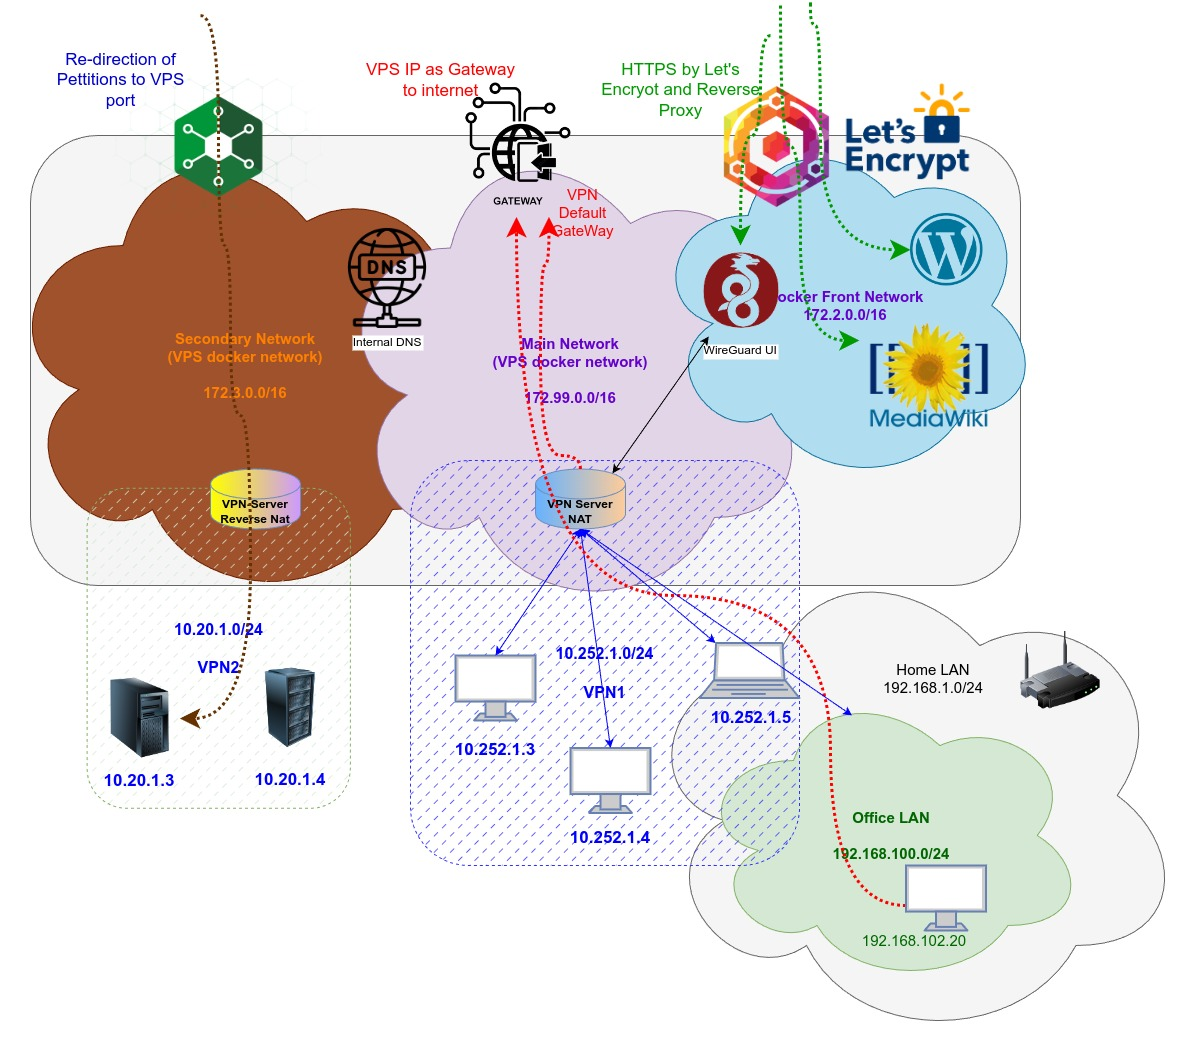
\includegraphics[width=1\textwidth]{./figuras/entorno-dockerNetworks.jpg}
\caption{Diagrama de interconexión de redes docker y servicios.}
\label{F:entorno-dockerNetworks}
\end{center}
\end{figure}
Por otra parte, si deseamos que nuestra VPN permita un acceso reverso, es decir enviar peticiones o trafico desde la red docker a nuestra IP en la VPN o nuestra LAN expuesta por dicha IP-vpn, no es posible la utilización de los servicios dockerizados, o el uso de la VPN como default gateway, ya que requiere implementar un Nat-reverso docker-network a VPN (véase flechas marrones figura \ref{F:entorno-dockerNetworks}),
o una configuración especifica (estática) de DMZ para permitir conexiones especificas a través del NAT.

Por ultimo para la interconexión de sedes, es indiferente, ya que las sedes pueden comunicarse a través de la red VPN, sin necesidad de pasar por las redes docker y no se ven afectadas por ningún tipo de NAT, únicamente es necesario tener un elemento conectado a la VPN en dichas LAN y la configuración adecuada.

\section{Caso desarrollado}
El caso desarrollado se ha centrado en la implementación de 3 VPN, focalizados en tres objetivos diferenciados (véase figura \ref{F:red_entorno_vpn}). 

Una primera VPN1 cuyo objetivo es la interconexión de elementos de la VPN(principal), la salida como puerta de enlace por el VPS y el acceso a servicios dockerizados internos (DNS, web, internos …). Una segunda VPN2 cuyo principal objetivo es la interconexión de LANs o enrutado. Y por último una tercera VPN3 que se puede acceder únicamente conectado a la VPN1 / VPN2, es decir una segunda capa VPN como explica el punto \ref{S:doble_layer} para aquellos servicios seguros y no disponibles desde la red principal del cloud.

\begin{figure}[!htb]
\begin{center}
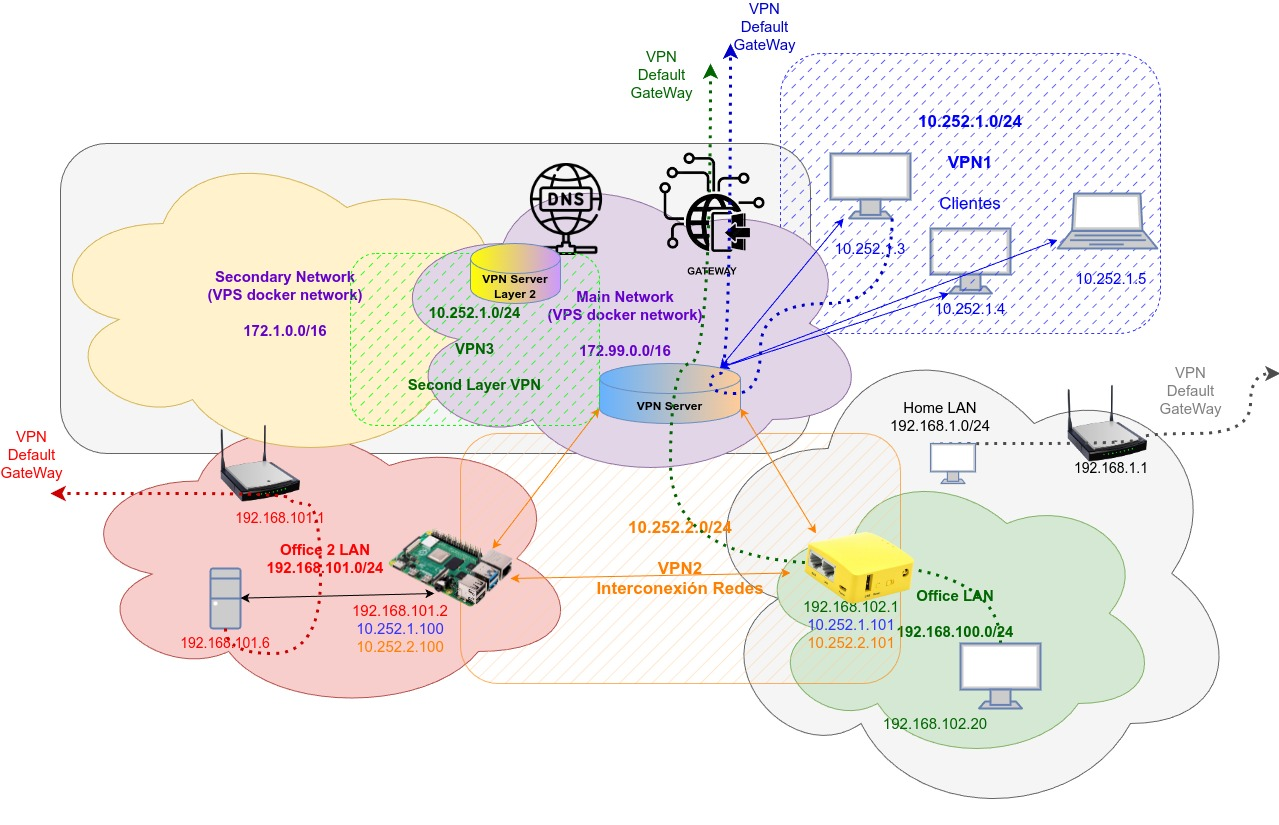
\includegraphics[width=1\textwidth]{./figuras/red_entorno_vpn}
\caption{VPNs, relación entre ellas VPS y clientes.}
\label{F:red_entorno_vpn}
\end{center}
\end{figure}

En el diagrama de la figura \ref{F:red_entorno_vpn} se muestra un ejemplo real donde tenemos 8 redes diferentes, 3 LAN, 3 VPN, y 2 redes docker:
\begin{itemize}
    \item VPN1 10.252.1.0/24 (azul) , cuyos clientes entunelan tráfico en esta red virtual privada, gestionada por el VPN server. Implementa un NAT masquerade de azul-morado, provee de acceso a internet y conectividad con los servicios dockerizdos de la red morada.
    \item VPN2 10.252.2.0/24 (naranja) , cuyos clientes entunelan tráfico en esta red virtual privada, gestionada por el VPN server. Provee conectividad de la red docker hacia las LAN de sedes y viceversa.
    \item Docker network 172.99.0.0/16 (morada), es una red privada de docker donde están la mayoría de  servicios docker del VPS. Permite enrutar tráfico a través del VPS al exterior. Las sedes tiene conectividad con dichos servicios vía VPN2 así como el resto de clientes de VPN1. Es la red principal del cloud-VPS.
    \item Office 2 LAN, 192.168.101.0/24 (rojo) compuesta por una oficina con router ADSL/fibra en la cual existe un dispositivo raspberry pi conectado a la VPN2. Permite acceder a la red morada (docker con servicios) y otras sedes (LAN verde oscuro). Ejemplo de casuística con default gateway por su propio router, no es por el VPS.
    \item Office LAN, 192.168.100.0/24 (verde oscuro) compuesta por una sede en casa con su propia LAN 192.168.1.0/24 adsl/fibra (gris) en la que se ha instalado un router wifi que habilita un NAT entre ambas e implementa un cliente vpn directo a la VPN2. Básicamente usa la red gris como infraestructura, se conecta vía VPN2 para enrutar todo el tráfico VPN-Red Docker hasta salir por el gateway del VPS. 
    \item  HomeLAN 192.168.1.0/24 (gris), LAN local de soporte a una red de oficina. Se puede observar como la red gris es independiente, no puede acceder a la red verde, ni ninguna otra red y su default gateway es su router, únicamente es usada como infraestructura.
    \item VPN Layer 2, VPN3 10.252.1.0/24 (verde claro), es una VPN únicamente accesible desde la red morada, es decir, se requiere de la VPN1 o estar en alguna LAN conectada a la VPN2 para poder acceder a ella. Similar a la VPN1-morada, realiza una conexión VPN3-amarilla, permitiendo acceder aquellos servicios dockerizados en la red docker interna amarilla y proveyendo de default gateway vía la red amarilla de docker.
    \item Second Docker net, 172.1.0.0/16 (amarilla) es otra red interna de docker la cual solo se puede acceder vía VPN3 que a su ves solo es accesible vía VPN1/VPN2. Es un caso de doble capa de VPN para acceder a los servicios.
    
    \item Elementos conectados a la VPN1, red azul, desde otros accesos, son terminales tunelados, es decir, su default gateway pasa a ser el VPS y usan el dns interno de la red morada docker. Tienen completa conectividad con los servicios de la red morada.
\end{itemize}

\section{Generalización de Casos}
Con el fin de explicar todas las posibilidades que brinda la nube generada en este documento, explicaremos los diferentes casos de uso general generar a través del diagrama de red de la figura \ref{F:red_entorno_vpn} y de la figura \ref{F:entorno-dockerNetworks} :
\begin{itemize}
    \item[--] Red verde oscura, es un ejemplo de despliegue por router portable, permite llegar a cualquier lugar y conectar por cable dicho router que genera un LAN autoconfigurada vía VPN2 a los servicios principales del VPS.
    \item[--] Red roja, es un ejemplo de sede conectada al VPS. No modifica la funcionalidad de la red, pero añade rutas estáticas de enrutado a través de un elemento conectado a la VPN2 en este caso una raspberry pi.
    \item[--] Red azul, es un ejemplo de VPN clásica, provee de acceso a internet vía VPS y permite la inter conectividad a diferentes redes (intranet). Aunque los clientes pertenecientes a dicha red (VPN1) pueden verse entre si, pero no son accesibles directamente desde el VPS ni exponen sus propias LAN.
    \item[--] Red naranja, en el diagrama \ref{F:red_entorno_vpn} es usada como infraestructura de interconexión entre sedes. Sin embargo puede ser utilizada como una VPN parcial similar a VPN1 pero sin usar el VPS como default gateway o utilizando los dns internos como alternativos, únicamente se utiliza para acceder a unos servicios concretos, especialmente si están en otras sedes.
    \item[--] Red morada, es una red virtual dentro del contexto del VPS. Es la \textbf{RED PRINCIPAL} de nuestro cloud, es decir la red troncal y en ella se sitúan los servicios dockerizados, está conectada a nivel bridge con el VPS por lo actúa como VPS-gateway y  como proveedor de dns internos. Aunque la gran mayoría de servicios son internos, un mínimo de ellos es publico (vpn server) o compartidos con otras redes docker.
    \item[--] Red verde clara, es un claro ejemplo de VPN múltiple layer, genera una VPN3 que solo es accesible una vez conectado a la VPN1 o VPN2.
     \item[--] Red amarilla, es un  caso de red aislada de docker, no accesible desde el exterior, requiere de una o mas VPN para ser accesible. 
    \item[--] Red gris, ejemplo de red de infraestructura sin acceso o interacción con las redes de cloud-VPS.
    \item[--] Red marrón, figura \ref{F:entorno-dockerNetworks} ejemplo de red docker interna con proxy de redirección, es decir, puede contener ciertos servicios expuestos, pero su principal función es exponer clientes VPN a través de un Nat-reverse y un reverse-Proxy en la ip del VPS.
    \item[--] Red azul claso, figura \ref{F:entorno-dockerNetworks} ejemplo de red docker con servicios públicos con su principal característica es un reverse-Proxy y let's encrypt para generar HTTPS en los servicios expuestos. Es una red aislada de la red principal (morada), aunque varios servicios puede estar en ambas redes como por ejemplo la front-ui de el servidor VPN.
\end{itemize}
